% Figure drawn for the vault (not in the course tex), section 44: a vector field on S^1, two pictures. Compile with the notes preamble.
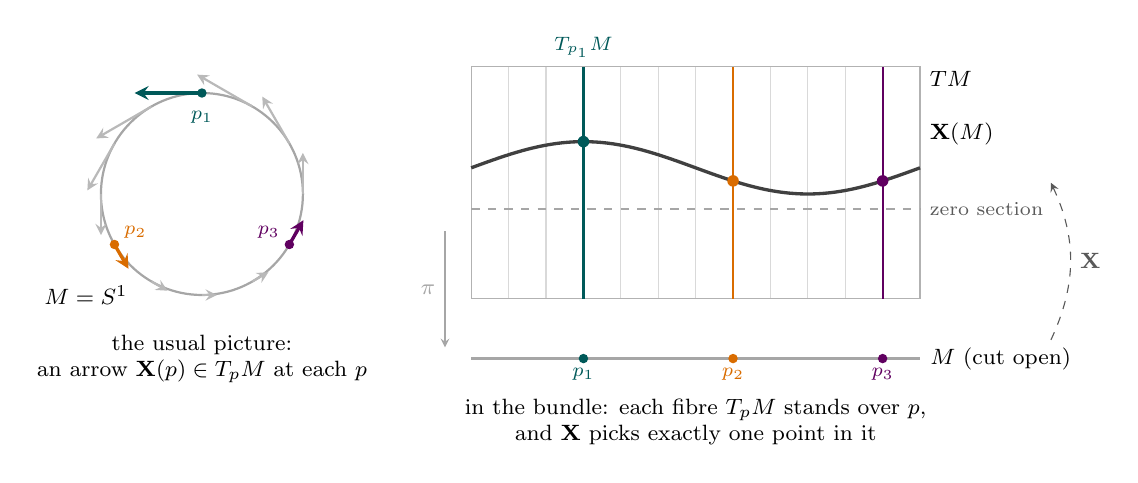
\begin{tikzpicture}[scale=0.95, >=stealth]
% ---------- left: the arrows on M = S^1 ----------
\def\R{1.35}
\draw[thick, gray!70] (0,0) circle (\R);
\node[font=\footnotesize] at (-1.55,-1.35) {$M = S^1$};
% faint arrows of the field X = c(t) d/dt, c(t) = 0.55 + 0.35 sin t
\foreach \a in {0,30,60,120,150,180,240,270,300} {
  \pgfmathsetmacro{\c}{0.55+0.35*sin(\a)}
  \draw[->, gray!55, thick] ({\R*cos(\a)},{\R*sin(\a)}) -- ++({-\c*sin(\a)},{\c*cos(\a)});
}
% three highlighted points
\foreach \a/\col/\lab in {90/teal!70!black/p_1, 210/orange!85!black/p_2, 330/violet!75!black/p_3} {
  \pgfmathsetmacro{\c}{0.55+0.35*sin(\a)}
  \fill[\col] ({\R*cos(\a)},{\R*sin(\a)}) circle (1.8pt);
  \draw[->, very thick, \col] ({\R*cos(\a)},{\R*sin(\a)}) -- ++({-\c*sin(\a)},{\c*cos(\a)});
  \node[font=\scriptsize, text=\col] at ({(\R-0.32)*cos(\a)},{(\R-0.32)*sin(\a)}) {$\lab$};
}
\node[font=\footnotesize, align=center] at (0,-2.2) {the usual picture:\\ an arrow $\mathbf{X}(p) \in T_pM$ at each $p$};
% ---------- right: the same field inside TM ----------
\begin{scope}[xshift=3.6cm, yshift=-0.2cm]
\def\W{6.0}
% fibres T_pM, vertical
\foreach \i in {0,...,12} { \draw[gray!30] ({\i*\W/12},-1.2) -- ({\i*\W/12},1.9); }
\draw[gray!60] (0,-1.2) rectangle (\W,1.9);
\node[font=\footnotesize, anchor=south west] at (\W,1.5) {$TM$};
% zero section
\draw[gray!70, dashed] (0,0) -- (\W,0) node[right, font=\scriptsize, text=gray!70!black] {zero section};
% the field as a curve: height = c(t), t = 360 x / W
\draw[very thick, black!75, domain=0:\W, samples=80] plot (\x, {0.55+0.35*sin(360*\x/\W)}) ;
\node[font=\footnotesize, anchor=west] at (\W,1.0) {$\mathbf{X}(M)$};
% base M, cut open
\draw[thick, gray!70] (0,-2.0) -- (\W,-2.0) node[right, font=\footnotesize, text=black, align=left] {$M$ (cut open)};
% the three points again
\foreach \a/\col/\lab in {90/teal!70!black/p_1, 210/orange!85!black/p_2, 330/violet!75!black/p_3} {
  \pgfmathsetmacro{\x}{\W*\a/360}
  \pgfmathsetmacro{\c}{0.55+0.35*sin(\a)}
  \draw[\col, thick] (\x,-1.2) -- (\x,1.9);
  \fill[\col] (\x,-2.0) circle (1.8pt) node[below, font=\scriptsize] {$\lab$};
  \fill[\col] (\x,\c) circle (2.2pt);
}
\node[font=\scriptsize, teal!70!black, anchor=south] at ({\W*90/360},1.9) {$T_{p_1}M$};
% the maps
\draw[->, gray!70] (-0.35,-0.3) -- node[left, font=\footnotesize] {$\pi$} (-0.35,-1.85);
\draw[->, dashed, gray!70!black] (\W+1.75,-1.75) to[bend right=25] node[right, font=\footnotesize] {$\mathbf{X}$} (\W+1.75,0.35);
\node[font=\footnotesize, align=center] at ({\W/2},-2.85) {in the bundle: each fibre $T_pM$ stands over $p$,\\ and $\mathbf{X}$ picks exactly one point in it};
\end{scope}
\end{tikzpicture}
